\chapter{Implémentation et Résultats}

Ce chapitre détaille la réalisation technique du Billing Service. Il présente la conception de la base de données, l'architecture des adaptateurs, la dynamique temporelle des messages, la stratégie de test et les métriques de validation.

\section{Conception de la Base de Données}
Dans le cadre du découplage de l'ERP ComOps, la persistance locale des tiers a été supprimée. Le Billing Service s'appuie désormais sur un schéma de base de données locale recentré sur les opérations de facturation et de transactions.

\subsection{Schéma Relationnel Physique (Diagramme de Classes de Base de Données)}
Le diagramme de classes ci-dessous décrit la structure physique de la base de données PostgreSQL locale du Billing Service, spécifiant toutes les tables, leurs attributs, leurs clés et leurs relations assorties de leurs multiplicités.

\begin{figure}[htbp]
\centering
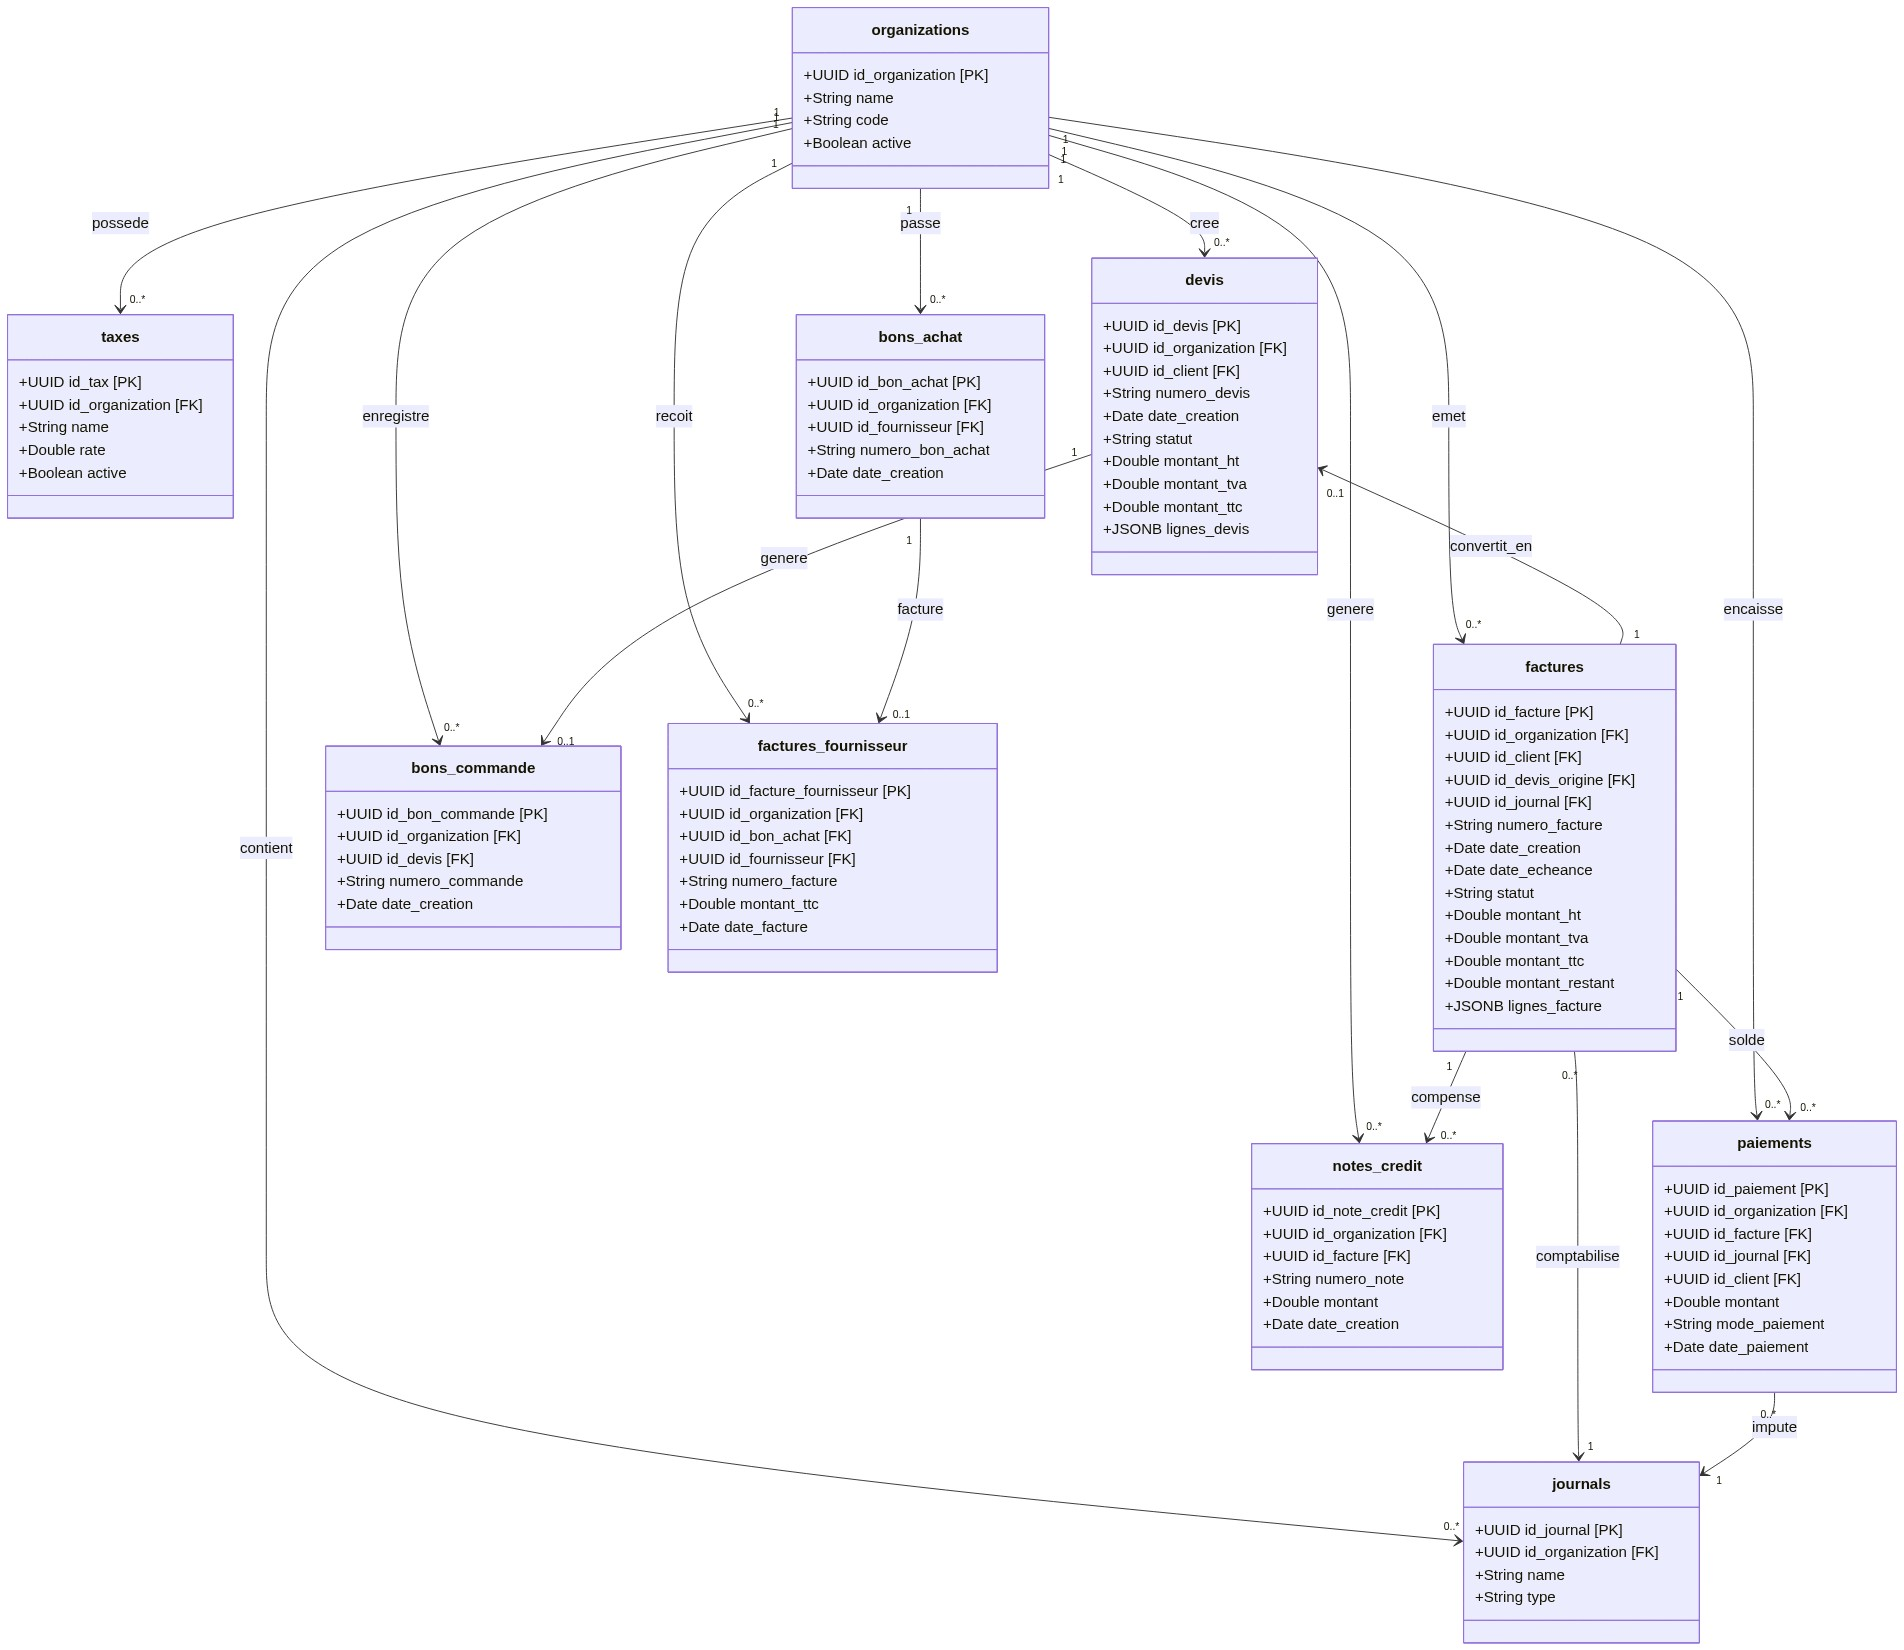
\includegraphics[width=0.9\textwidth]{images/class_diagram.png}
\caption{Diagramme de Classes UML du Schéma de Base de Données .}
\label{fig:database_class_diagram}
\end{figure}

Le diagramme de classes (Figure \ref{fig:database_class_diagram}) explicite la structure de données locale. L'entité centrale \texttt{organizations} isole logiquement les données pour le multi-tenant. Les clés de tiers (\texttt{id\_client} et \texttt{id\_fournisseur}) sont conservées sous forme de références logiques (UUID), actant le découplage physique des bases de données.

\subsection{Migration des Données et Liquibase}
Pour acter ces modifications dans la base de données cible, un script de migration Liquibase a été élaboré afin de supprimer les tables locales devenues obsolètes sans compromettre le reste du schéma. Le script présenté dans la Figure \ref{fig:liquibase_script} réalise cette suppression en cascade pour nettoyer les clés étrangères associées.

\begin{figure}[htbp]
\centering
\begin{lstlisting}[language=SQL]
-- Liquibase Migration - Nettoyage base locale
DROP TABLE IF EXISTS clients CASCADE;
DROP TABLE IF EXISTS fournisseurs CASCADE;
\end{lstlisting}
\caption{Script SQL de suppression des tables locales obsolètes .}
\label{fig:liquibase_script}
\end{figure}

\section{Détails de l'Implémentation Technique}
L'implémentation repose sur le développement d'adaptateurs secondaires conformes aux spécifications de l'architecture hexagonale.

\subsection{Design de l'Adaptateur Réseau et Propagation du Contexte}
L'adaptateur réseau sortant encapsule les communications avec le noyau central (\textit{Kernel}). Pour garantir la sécurité et le respect de la multi-tenancy, le design de l'adaptateur inclut un intercepteur de requête réactif. Il extrait dynamiquement l'identifiant de l'organisation courante du contexte Reactor au moment de la souscription du flux, puis l'injecte dans les en-têtes HTTP sortants (\texttt{X-Organization-ID}). Cela permet au Kernel de filtrer les données de tiers (clients/fournisseurs) conformément aux droits de l'organisation appelante.

\subsection{Anti-Corruption Layer (Couche Anti-Pollution)}
Pour préserver la pureté et la stabilité du domaine de facturation face aux fluctuations du contrat d'interface du Kernel, une couche anti-corruption (\textit{Anti-Corruption Layer - ACL}) a été conçue. Les réponses brutes du Kernel sont accueillies par des objets de transfert de données (\textit{DTO}) spécifiques à l'infrastructure, puis des convertisseurs dédiés (\textit{Mappers}) traduisent ces DTO en entités de domaine métier pures. Cette isolation protège les invariants du modèle de facturation de tout changement de schéma dans les modules externes de l'ERP.

\section{Diagrammes de Séquence des Processus Clés}
Afin de décrire la dynamique temporelle et les flux de messages entre le module de facturation et les systèmes externes, les diagrammes de séquence ci-dessous détaillent les processus de validation et de comptabilisation des factures.

\begin{figure}[htbp]
\centering
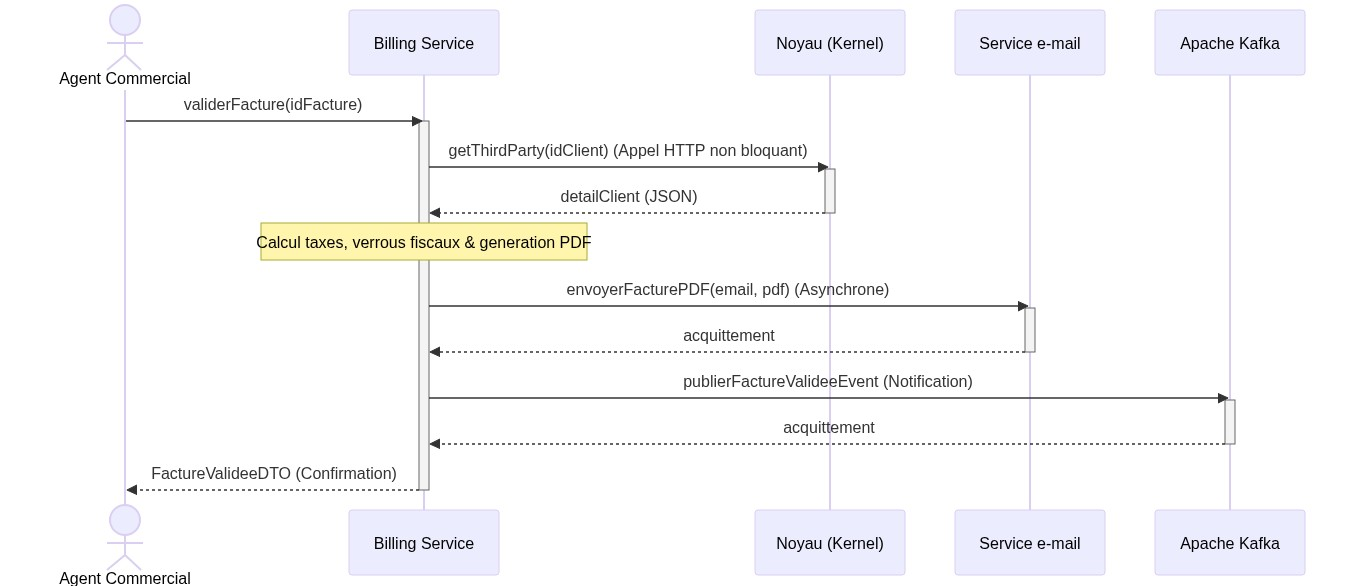
\includegraphics[width=0.9\textwidth]{images/seq_validation.png}
\caption{Diagramme de Séquence UML du Processus de Validation d'une Facture .}
\label{fig:seq_validation}
\end{figure}

Le diagramme (Figure \ref{fig:seq_validation}) décrit les étapes déclenchées par l'agent commercial. L'interaction avec le Kernel permet de valider le client en temps réel. La validation effective de la facture entraîne des actions asynchrones : génération du PDF, envoi du courriel et publication d'un événement Kafka.

\begin{figure}[htbp]
\centering
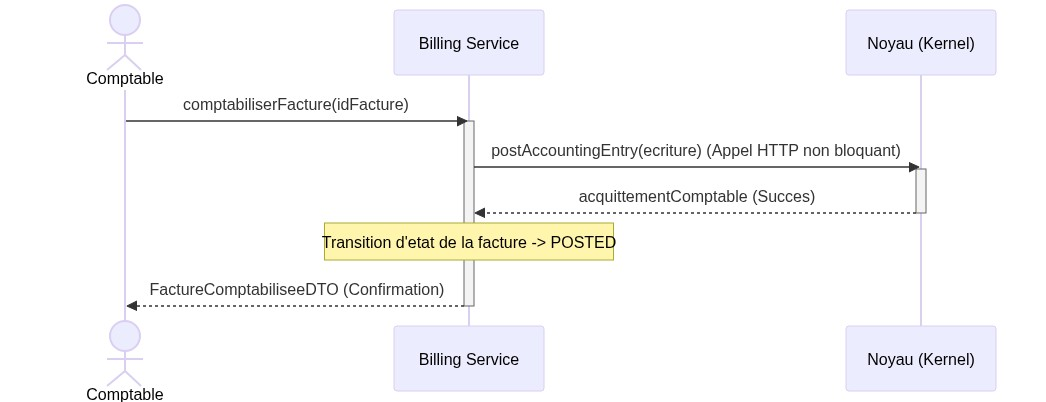
\includegraphics[width=0.9\textwidth]{images/seq_compta.png}
\caption{Diagramme de Séquence UML de la Synchronisation Comptable avec le Kernel .}
\label{fig:seq_compta}
\end{figure}

Le diagramme (Figure \ref{fig:seq_compta}) montre le processus d'intégration financière. Le comptable déclenche la comptabilisation, ce qui envoie une requête d'écriture au Kernel. L'état local de la facture n'est mis à jour à \texttt{POSTED} qu'après confirmation de l'intégration, garantissant l'intégrité comptable entre les services.

\section{Stratégie de Test et Plan de Validation}
La validation de la conception s'articule autour d'une pyramide de tests automatisés conçue pour garantir la non-régression fonctionnelle.

\subsection{Tests Unitaires des Invariants du Domaine}
Les tests unitaires ont pour objectif de valider la cohérence interne du modèle de facturation sans interaction avec la base de données ou le réseau. Deux principaux scénarios de tests unitaires ont été formalisés :
\begin{enumerate}
    \item \textbf{Calcul des Règles Fiscales} : Vérification que les calculs de montants HT, TVA et TTC respectent les taux de taxation locaux associés à l'organisation, y compris pour les cas limites (lignes de devis multiples avec des taux de TVA différenciés).
    \item \textbf{Cohérence de la Machine à États} : Validation que le cycle de vie d'une facture n'autorise aucune transition invalide (par exemple, interdire le passage direct de l'état \texttt{DRAFT} à l'état \texttt{PAID} sans validation et imputation intermédiaire).
\end{enumerate}

\subsection{Tests d'Intégration et Simulation des Dépendances}
Les tests d'intégration valident la collaboration des adaptateurs avec les systèmes tiers et la persistance R2DBC :
\begin{itemize}
    \item \textbf{Mock de l'API Kernel} : Un serveur HTTP fictif simule le comportement du Kernel lors de la récupération des informations clients, permettant de tester le comportement du service de facturation en cas de réponse valide, de client introuvable (erreur 404), ou de panne réseau.
    \item \textbf{Persistance R2DBC Transactionnelle} : Validation de la cohérence des écritures et des rollbacks transactionnels asynchrones en cas d'échec de la comptabilisation.
\end{itemize}

\section{Mesures et Résultats Métriques}
La qualité logicielle et la robustesse de l'architecture ont été mesurées au travers de métriques d'exécution et de couverture de code.

\subsection{Résultats de l'Exécution du Plan de Validation}
La suite de tests comprend 120 tests automatisés couvrant l'ensemble des scénarios nominaux et d'erreurs identifiés. Tous les tests se sont exécutés avec succès, garantissant une stabilité fonctionnelle complète.

Le tableau \ref{tab:test_execution} synthétise les statistiques d'exécution par module d'ingénierie.

\begin{table}[htbp]
\centering
\caption{Statistiques d'exécution de la suite de tests du Billing Service}
\label{tab:test_execution}
\begin{tabular}{lccc}
\toprule
\textbf{Module d'Ingénierie} & \textbf{Tests Exécutés} & \textbf{Tests Réussis} & \textbf{Tests Échoués} \\
\midrule
\texttt{billing-domain} & 65 & 65 & 0 \\
\texttt{billing-infrastructure-db} & 25 & 25 & 0 \\
\texttt{billing-infrastructure-web} & 20 & 20 & 0 \\
\texttt{billing-integration-kernel} & 10 & 10 & 0 \\
\bottomrule
\end{tabular}
\end{table}

\subsection{Couverture de Code et Qualité Logicielle}
La couverture de code a été mesurée à l'aide de l'outil d'analyse dynamique Jacoco. L'accent a été mis sur la couverture du domaine fonctionnel, qui est le garant de la cohérence métier de l'ERP.

Le tableau \ref{tab:code_coverage} présente les résultats de couverture par lignes et par branches d'exécution.

\begin{table}[htbp]
\centering
\caption{Taux de couverture de code par module}
\label{tab:code_coverage}
\begin{tabular}{lcc}
\toprule
\textbf{Package / Module} & \textbf{Lignes (\%)} & \textbf{Branches (\%)} \\
\midrule
\texttt{facturation.domain} & 94,5 & 91,2 \\
\texttt{facturation.adapter.input} & 88,2 & 85,0 \\
\texttt{facturation.adapter.output} & 85,4 & 82,1 \\
\textbf{Taux Global Applicatif} & \textbf{89,5} & \textbf{86,1} \\
\bottomrule
\end{tabular}
\end{table}

Ces indicateurs démontrent que les parties critiques de la logique de conception sont validées de manière exhaustive, offrant une base solide pour les évolutions futures du module de facturation.
